\section{Proposal}

With Swift, the available access control mechanism is  ACL ( access Control List) which specify who can or cannot access an object or a file. In this approach, if someone can access a document, he/she gets the full content of the document which is an all or nothing approach.  Figure \ref{fig:swift_file} and \ref{fig:zwift_file}  illustrates the situation where in the former case, a file is accessed in all / nothing approach and in the later case the file can be selectively accessed by different users. But we believe that   zerovm enables more sophisticated cases which require more flexible access control than the ACL. For example,  a hospital that stores patient medical record in the cloud,  wants all its doctor, nurse or patient access the partial content based on the available role of the requester.  So, along with the content, the owner (in this case, the hospital) of an object/file may need to specify who can access how much of the content.

\begin{figure}[h!] 
\label{fig:swift_file}
  \centering
    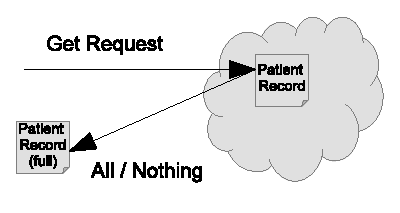
\includegraphics[width=0.3\textwidth]{eps/swift_file}
 \caption{A picture of a gull.}
\end{figure}

\begin{figure}[h!]
\label {fig:zwift_file} 
  \centering
    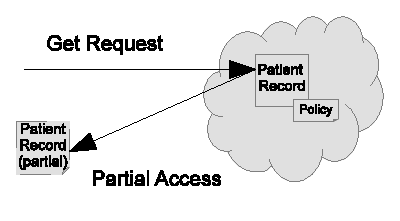
\includegraphics[width=0.3\textwidth]{eps/zwift_file}
 \caption{A picture of a gull.}
\end{figure}




listing \ref{patient Record}, shows a sample file to be stored in the object store. For our example, we specify three different user roles namely, doctors, patient, and nurse.
A sample policy to be specified by the content owner is shown in listing \ref{content policy}.


\begin{listing}
\begin{minted}[frame=single,
               framesep=3mm,
               linenos=true,
               xleftmargin=21pt,
               tabsize=2]{js}
{
 "medical_record": {
 "Personal_information": {
	    "Name": "Monica Latte",              
           "Gender": "Female",
           "Contact By": "Phone"
       },
       "identification": {
         "Soc_Sec_No": "444-444",
         "Patient_ID": "0000-44"
       },
      "physical_exam": {
	  "appearance": "well developed",
	  "eyes": "conjunctiva"
	},
       "Medications": [
            "PRINIVIL TABS 20 MG ",
            "Last Refill: #30 x 2 "
        ]    
      
    }
}

\end{minted}
\caption{Content of a file in the Object Storage} 
\label{patient Record}
\end{listing}

\begin{enumerate}

  \item  personal information as specified by jsonpath //personal\_information (shown in line 2 to 7), should be labeled 'personal' and only the owner of the file should be able access objects labeled personal .

  \item Identification information as specified by jsonpath //identification (shown in lines between 8 and 11), should be labeled 'billing' and only 'accountant' should be able to access it.

  \item  doctor  can access all json objects if it is not labeled 'personal' or 'billing'
\end{enumerate}

Now, whenever a user having role doctor request to get the file, he would be able to access the content as specified in listing \ref{request response} 

\begin{listing}
\begin{minted}[frame=single,
               framesep=3mm,
               linenos=true,
               xleftmargin=21pt,
               tabsize=2]{js}
{
 "medical_record": { 
      "physical_exam": {
	  "appearance": "well developed",
	  "eyes": "conjunctiva"
	},
  "Medications": [
            "PRINIVIL TABS 20 MG ",
            "Last Refill: #30 x 2 "
        ]   
}  
}

\end{minted}
\caption{Content of  Medical Record Object as Accessed by a User Having Doctor Role} 
\label{request response}
\end{listing}

To sum up our proposal of Content Based Access Control, we want to achieve following:


\begin{enumerate}

  \item Attach a policy with file/object stored in swift. When the file is accessed, instead of having the full content, the requester gets selective content based on this acting role. This case is explained in the above section.


\item Attach a policy at the container label 

\end{enumerate}









